% !TeX encoding = UTF-8
% !TeX spellcheck = de_DE

%% Dies gibt Warnungen aus, sollten veraltete LaTeX-Befehle verwendet werden
\RequirePackage[l2tabu, orthodox]{nag}

\documentclass[utf8,biblatex]{lni}
\bibliography{lni-paper-example-de}

%% Schöne Tabellen mittels \toprule, \midrule, \bottomrule
\usepackage{booktabs}

%% Zu Demonstrationszwecken
\usepackage[math]{blindtext}
\usepackage{mwe}

%% BibLaTeX-Sonderkonfiguration,
%% falls man schnell eine existierende Bibliographie wiederverwenden will, aber nicht die .bib-Datei händisch anpassen möchte.
%% Bitte \iffalse und \fi entfernen, dann ist diese Konfiguration aktiviert.

\iffalse
\AtEveryBibitem{%
  \ifentrytype{article}{%
  }{%
    \clearfield{doi}%
    \clearfield{issn}%
    \clearfield{url}%
    \clearfield{urldate}%
  }%
  \ifentrytype{inproceedings}{%
  }{%
    \clearfield{doi}%
    \clearfield{issn}%
    \clearfield{url}%
    \clearfield{urldate}%
  }%
}
\fi

\begin{document}
%%% Mehrere Autoren werden durch \and voneinander getrennt.
%%% Die Fußnote enthält die Adresse sowie eine E-Mail-Adresse.
%%% Das optionale Argument (sofern angegeben) wird für die Kopfzeile verwendet.
\title[WSL]{Windows Subsystem for Linux}
%%%\subtitle{Untertitel / Subtitle} % falls benötigt
\author[Marius Rusu \and Julia Sommer]
{Marius Rusu\footnote{Ludwig-Maximilian-Universität München, Fakultät für Informatik, Oettingenstraße 67, 80538 München, Deutschland \email{rusu.marius97@gmail.com}} \and
 Julia Sommer\footnote{Technische Universität München, Fakultät für Informatik, Boltzmanstraße 3, 85748 Garching, Deutschland \email{sommerjulia99@gmail.com}}}
\startpage{11} % Beginn der Seitenzählung für diesen Beitrag
\editor{Herausgeber et al.}    % Namen der Herausgeber
\booktitle{Name-der-Konferenz} % Name des Tagungsband
\year{2017}
%%%\lnidoi{18.18420/provided-by-editor-02} % Falls bekannt
\maketitle

\begin{abstract}
The Windows Subsystem for Linux is a new feature that enables running native Linux command-line tools directly on Windows. This paper shall investigate its architecture and implementation and compare it to other common Linux virtualizations.
\end{abstract}

\begin{keywords}
Windows Subsystem for Linux \and Virtualization
\end{keywords}

\section{Microsoft's reasons for WSL}

Many programmers that work with open source, Linux based tools such as Pearl and Python are struggeling on Windows. Especially when it comes to server infrastructure, programmers work with applications native to Linux since most of the Servers are also powered by Linux. Those applications unsually do not work great on Windows and programmers depend on workarounds like Containers and Virtual Machines. Alternatively, they switch to Linux or other Unix based operating systems. \footnote{https://blogs.windows.com/buildingapps/2016/03/30/run-bash-on-ubuntu-on-windows/#xKYy1Osl93c7kTAv.97}

Based on their feedback, Microsoft firstly \glqq made investments that improve cmd, PowerShell, and many other command-line tools and developer scenarios [and secondly] decided to grow [their] command line family by adding real, native Bash and with it support for Linux command-line tools which run directly on Windows in an environment that behaves like Linux \glqq \footnote{https://blogs.windows.com/buildingapps/2016/03/30/run-bash-on-ubuntu-on-windows/#xKYy1Osl93c7kTAv.97}
To accomplish this, Microsoft worked together with Cononical and published the Windows Subsystem for Linux running Ubuntu in April 2016. \footnote{https://blogs.windows.com/buildingapps/2016/03/30/run-bash-on-ubuntu-on-windows/#xKYy1Osl93c7kTAv.97}


\section{WSL - What is it?}
The following will provide information about the Windows Subsystem for Linux, based on Microsoft's publication.

\subsection{General Concept}
"Windows Subsystem for Linux is a collection of [user mode and kernel mode] components that enable native Linux ELF64 binaries to run on Windows."\footnote{} User mode applications are low privileged and depend on system calls to operate on kernel mode. Only in kernel mode low level operations directly handled by the operating system can be executed. In WSL we have the bash.exe running in user mode and initiating the Linux Instance. Further this instance submits, if necessary, native Linux system calls to be executed on a Linux Kernel. However, by virtualizing a Linux Kernel interface those system calls can be executed directly on the Windows Kernel. This virtualization is done by the LXCore/LXSS running in kernel mode.\footnote{ https://blogs.msdn.microsoft.com/wsl/2016/04/22/windows-subsystem-for-linux-overview/, 18.04.2018 19:32 Uhr}

\subsection{Basic Architecture}

\begin{comment}

(Windows Subsystem for Linux \glqq is primarily comprised of: 
\begin{enumerate}
    \item User mode session manager service [...]
    \item Pico provider drivers [...]
    \item Pico processes [...] \grqq\footnote{}
\end{enumerate})

\end{comment}

Windows Subsystem for Linux is primarily comprised of: 
\begin{enumerate}
    \item LX Session Manager
    \item LXCore/LXSS
    \item Pico processes\footnote{}
\end{enumerate}

\begin{figure}
  \centering
  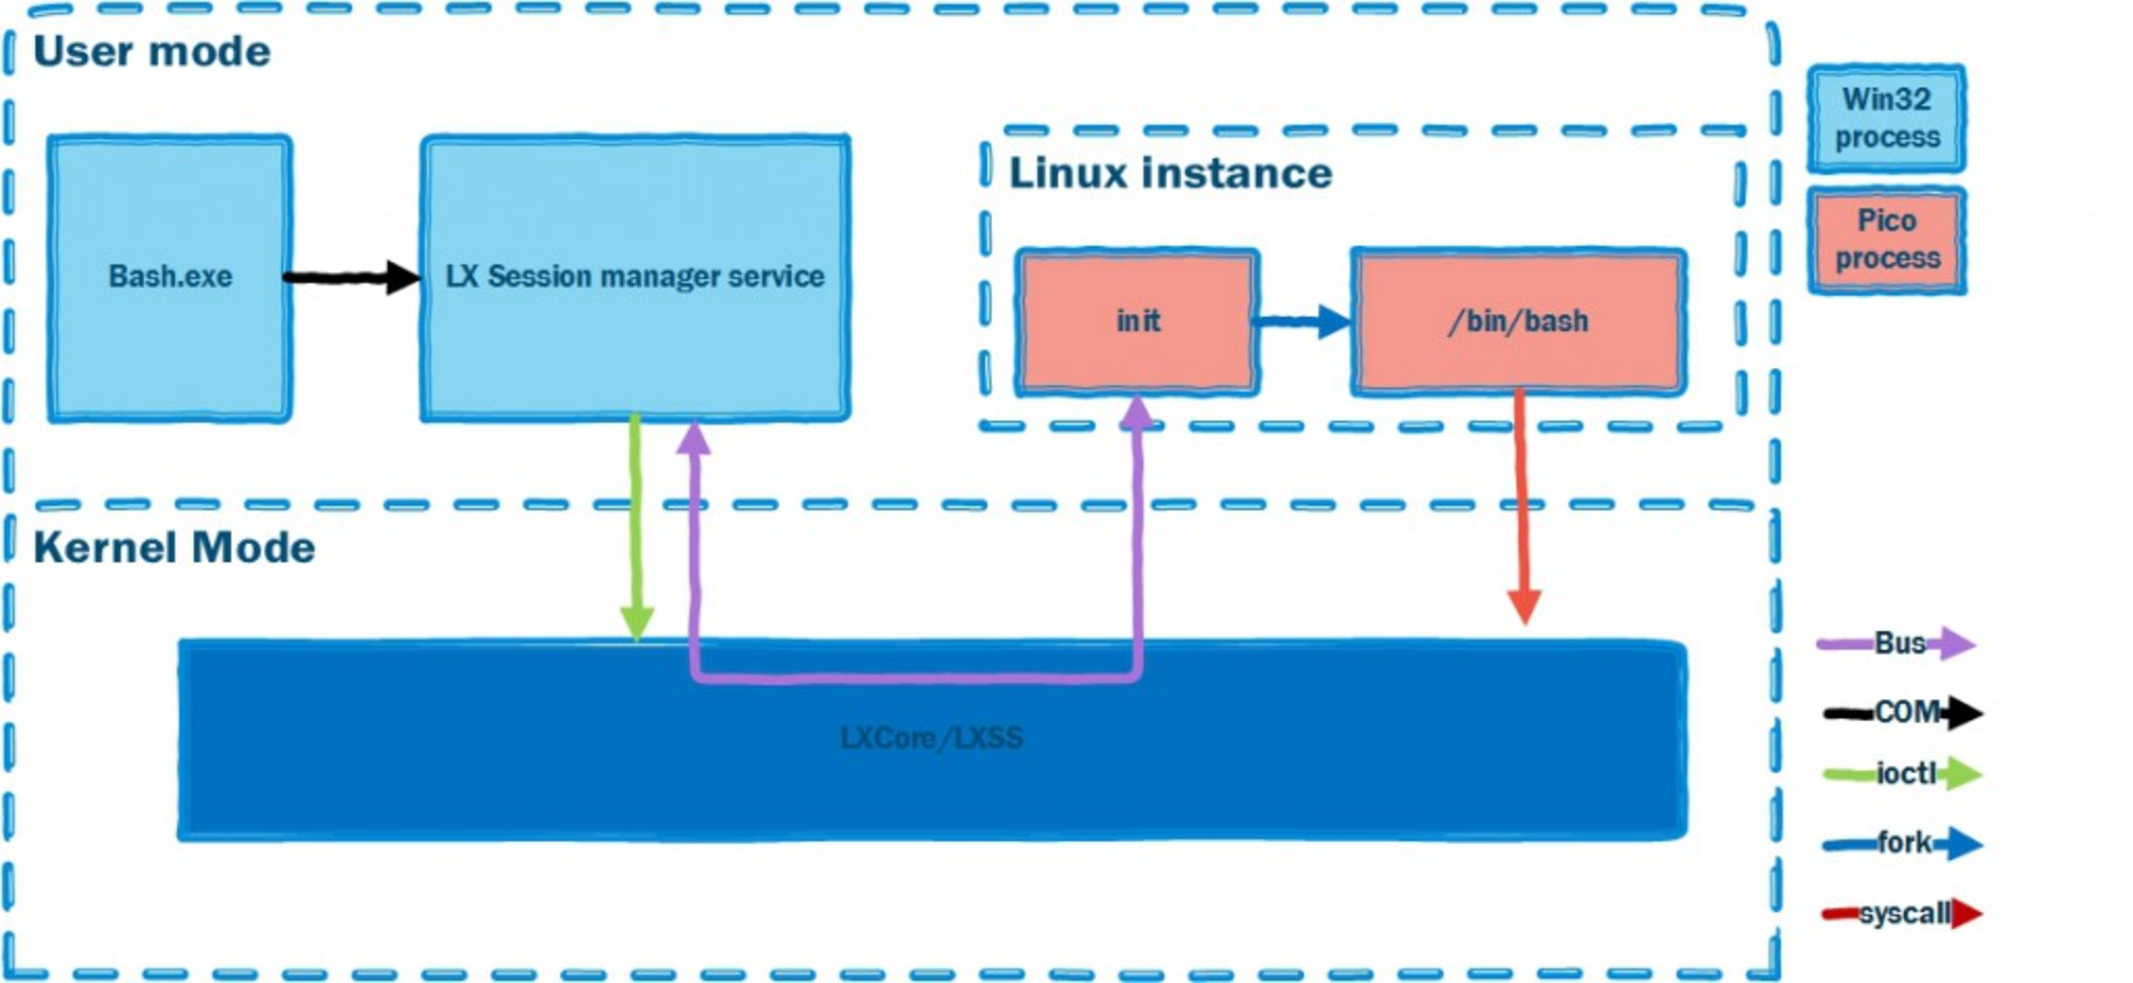
\includegraphics[width=1\textwidth]{WSL Architecture.pdf}
  \caption{Components of WSL}
  \label{img:architecture}
\end{figure}


As depicted in the image above, the user initiates the Windows Subsystem for Linux by launching the bash.exe on Windows. This application then calls the LXCore/LXSS (green arrow) which is a "[...] driver behaving like a Linux Kernel and working in coordination with the Windows Kernel. [The Driver] would then spin up a native Linux process [being] /bin/bash (purple arrow)."\footnote{https://blogs.msdn.microsoft.com/wsl/2016/05/23/pico-process-overview/} All other Linux processes run under /bin/bash in the so called Linux Instance that "[...] you can think of as [...] a container or a virtualized operating system environment." \footnote{https://blogs.msdn.microsoft.com/wsl/2016/05/23/pico-process-overview/}

\glqq By wrapping unmodified Linux binaries into pico processes we enable Linux system calls to be directed into the Windows kernel.\grqq \footnote{} A pico process itself is an empty process, as far as the Windows kernel is concerned and therefore cannot be handled by the Windows kernel but instead is redirected to the LXCore/LXSS (red arrow).\footnote{https://blogs.msdn.microsoft.com/wsl/2016/05/23/pico-process-overview/}
It is safe to say, that \glqq pico processes and drivers [LXCore/LXSS] provide the foundation for the Windows Subsystem for Linux [...]. \grqq \footnote{}

\begin{comment}

As mentioned, those system calls are native Linux system calls. Therefore the LXCore/LXSS being an emulation of the Linux Kernel\footnote{https://blogs.msdn.microsoft.com/wsl/2016/04/22/windows-subsystem-for-linux-overview/} map those system calls to an equivalent Windows system call to run on the Windows Kernel. However this is not always possible e.g. the operation fork() does not have a Windows equivalent. In that case the Windows Kernel has to handle the system call directly and satisfy its needs.

\end{comment}

\subsection{Implementation of its components}

\glqq The pico process concept originated in MSR [Microsoft Research] as part of the Drawbridge project. A goal of this project was to implement a lightweight way to run an application in an isolated environment, with the application’s OS dependencies decoupled from the underlying host OS\glqq \footnote{https://blogs.msdn.microsoft.com/wsl/2016/05/23/pico-process-overview/} This was achieved, not by a Virtual machine, which would be too resource consuming but by \glqq run[ning] the target application and OS entirely within the user-mode address space of a single process on the host OS. \glqq \footnote{https://blogs.msdn.microsoft.com/wsl/2016/05/23/pico-process-overview/} \glqq The Drawbridge pico process is a lightweight, secure isolation container. It is built from an OS process address space, but with all traditional OS services removed. [...] All ABI [Application binary interface] calls are serviced by the security monitor, which plays a role similar to the hypervisor or VM monitor in traditional hardware VM designs.\glqq \footnote{https://www.microsoft.com/en-us/research/project/drawbridge/?from=http\%3A\%2F\%2Fresearch.microsoft.com\%2Fen-us\%2Fproject s\%2Fdrawbridge\%2F}

In case of Windows subsystem for Linux this is exactly the point where pico processes are redirected to the LXCore/LXSS. \glqq The drivers do not contain code from the Linux kernel but are instead a clean room implementation of Linux-compatible kernel interfaces. [..] Where possible, lxcore.sys translates the Linux syscall to the equivalent Windows NT call which in turn does the heavy lifting. Where there is no reasonable mapping the Windows kernel mode driver must service the request directly.\glqq \footnote{} Since the Windows Kernel was originally designed to support multiple operating systems, Microsoft had to \glqq [dust] [...] of old functionality, [enhance] it for performance and correctness and it was able to go right away.\glqq \footnote{https://blogs.msdn.microsoft.com/wsl/2016/05/23/pico-process-overview/} Those changes in the Windows kernel enable it to execute even foreign operations like fork(). Windows applications however do not have access to those specific Linux system calls. \footnote{}

\glqq The File system support in WSL was designed to meet two goals:
\begin{enumerate}
    \item Provide an environment that supports the full fidelity of Linux file systems
    \item Allow interoperability with drives and files in Windows
\end{enumerate}\footnote{https://blogs.msdn.microsoft.com/wsl/2016/04/22/windows-subsystem-for-linux-overview/}

\glqq VolFs is a file system that provides full support for Linux file system features, including Linux permissions that can be modified through operations such as chmod and chroot [etc].\glqq \footnote{https://blogs.msdn.microsoft.com/wsl/2016/04/22/windows-subsystem-for-linux-overview/} Due to the fact that VolFs file system is not able to interoperate with Windows, a second file system named DriveFs is implemented. \glqq All fixed Windows volumes are mounted under /mnt [...] where users can access all Windows files.\glqq \footnote{https://blogs.msdn.microsoft.com/wsl/2016/04/22/windows-subsystem-for-linux-overview/} To make this possible the DriveFs file system meets Windows requirements such as legal file names and Windows security but looses some of the Linux features.

\section{Alternatives to Windows Subsystem for Linux}
The following will discuss other possibilities of running Linux on Windows and compare them to the Windows Subsystem for Linux.

\subsection{Classical approach to virtualization}

\subsection{Virtualization via Virtual Machine}

\begin{figure}
  \centering
  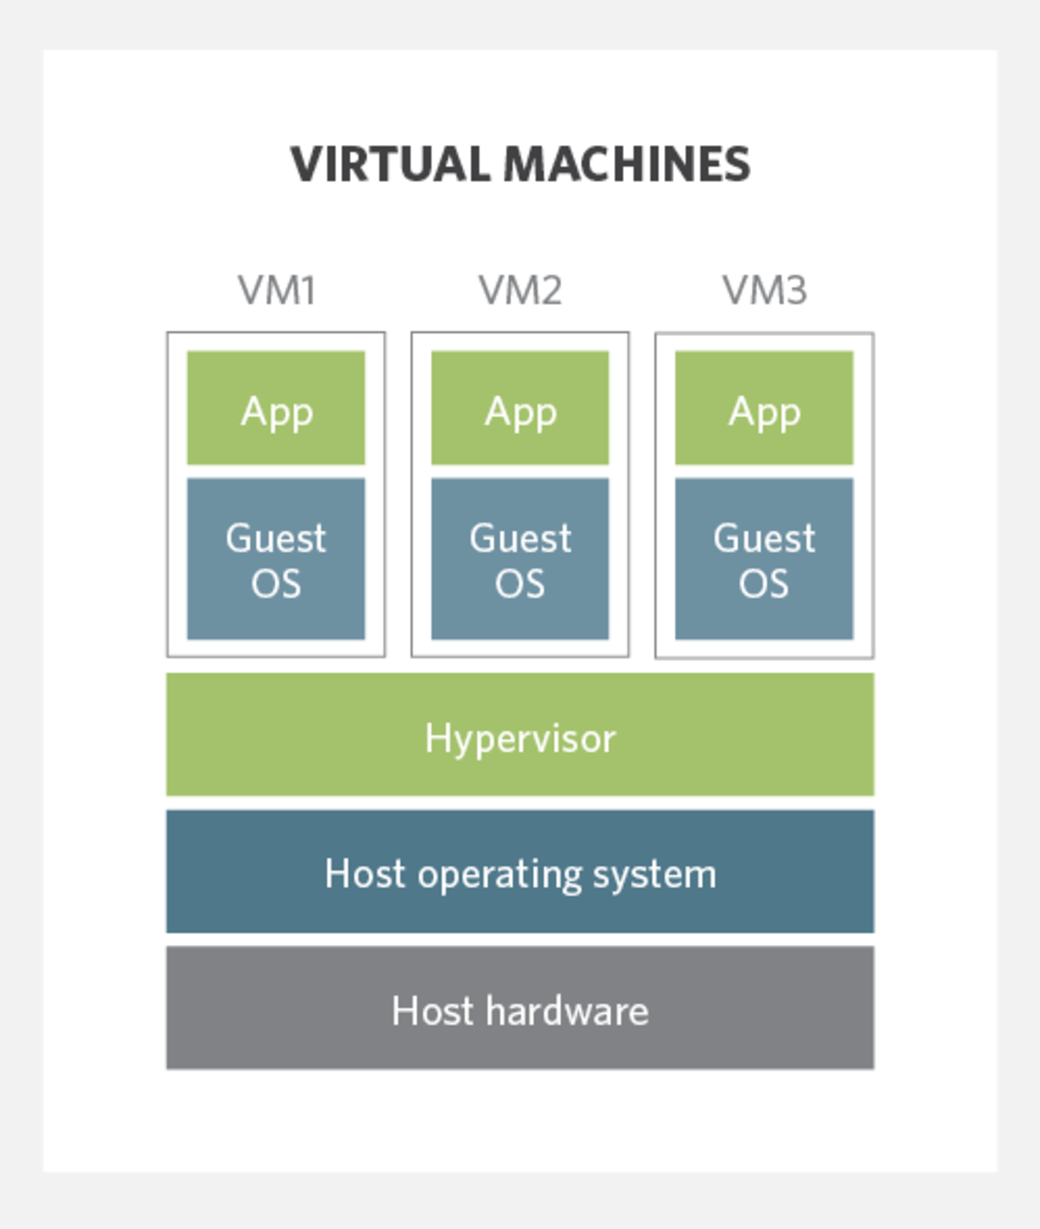
\includegraphics[width=0.5\textwidth]{VM.pdf}
  \caption{Virtual Machine Overview}
  \label{img:vm}
\end{figure}

\glqq The virtual machine concept allows the same computer to be shared as if it were several. IBM defined the virtual machine as a fully protected and isolated copy of the underlying physical machine’s hardware. \glqq\footnote{R. Rose, \glqq Survey of System Virtualization Techniques \glqq https://ir.library.oregonstate.edu/concern/parent/t148fh24b/file_sets/0r967383v} 
Therefore it is possible to run different applications on different operating systems at the same time on the same hardware as depicted in the image above. \glqq The VMM [Virtual Machine Monitor] is the software component that hosts guest virtual machines.\glqq \footnote{https://ir.library.oregonstate.edu/concern/parent/t148fh24b/file_sets/0r967383v} According to Prof. Dr. Kranzmüller and Dr. Danciu the Virtual Machine Monitor is firstly responsible for coordinating the access of the guest operation systems on the host's hardware and secondly for handling traps. Traps are created when a guest operating system is trying to execute a privileged operation. In that case, the Virtual Machine Monitor emulates its function in order to be executed on the host operating system. \footnote{Skript!}

\begin{figure}
  \centering
  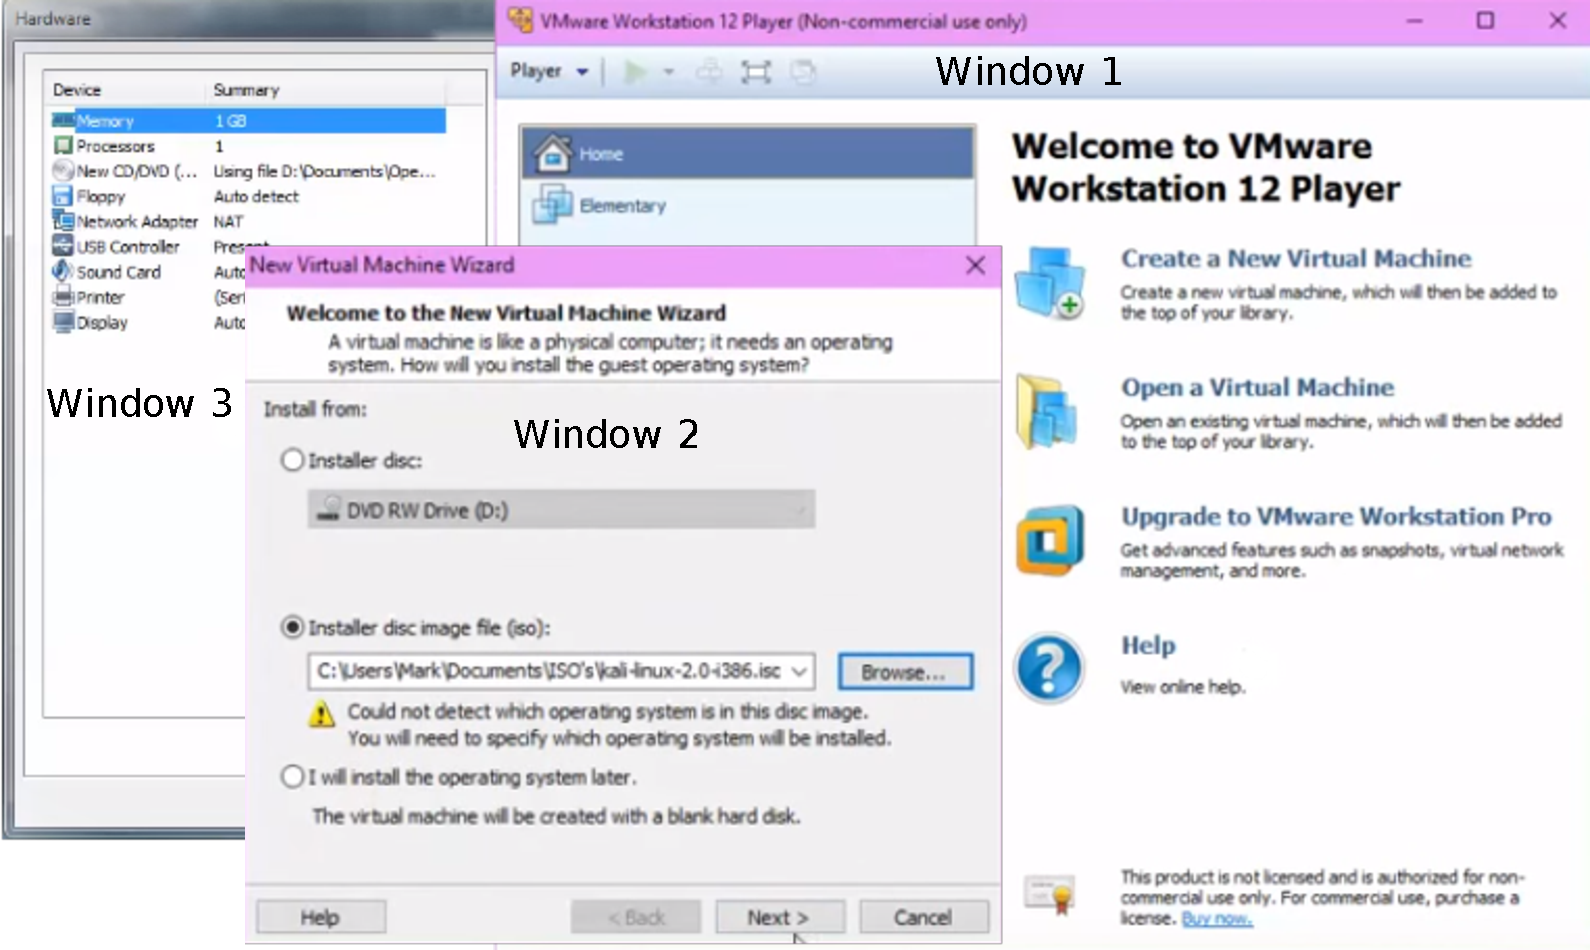
\includegraphics[width=0.9\textwidth]{VMware Player.pdf}
  \caption{VMware Player's graphic interface}
  \label{img:VMwarePlayer}
\end{figure}

A common tool for creating a virtual machine is VMware Player by VMware Inc. This application hides all the work of the Virtual Machine Monitor and comes with a graphic interface that can be seen above (Window 1). For creating a new virtual machine an image file of the guest operating system is needed, which can be either on a disc or downloaded from the internet (Window 2). After this, the user can decide on how many ressources, e.g. memory space and CPU cores the new virtual machine can use (Window 3). Finally, VMware Player launches the guest operating system in a new window as a fully functional and isolated operating system.

\subsection{Virtualization via Container}

\begin{figure}
  \centering
  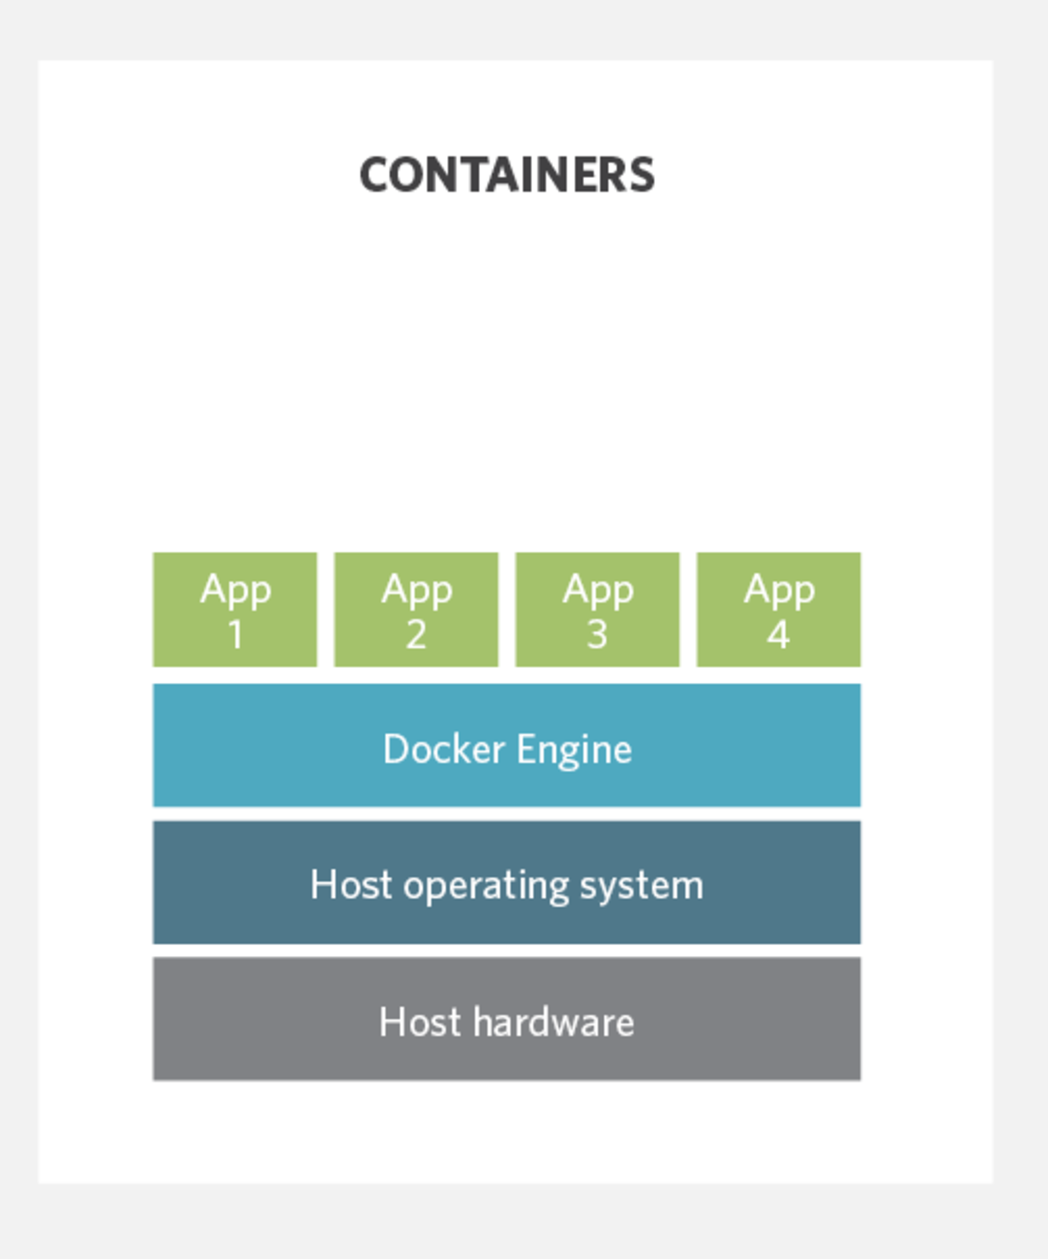
\includegraphics[width=0.5\textwidth]{Container.pdf}
  \caption{Container Overview}
  \label{img:container}
\end{figure}

Rather than virtualizing the hardware, containers use the host operating system and share its kernel. According to V. Badola containers are stripped down Virtual Machines running just enough software to deploy an application. \footnote{https://cloudacademy.com/blog/container-virtualization/} Instead of a Virtual Machine Monitor there is a container engine running on top on the host operating system which can be seen in the image above. \glqq A container engine is a managed environment for deploying containerized applications. The container engine allocates cores and memory to containers [and] enforces spatial isolation and security [...] \glqq \footnote{https://insights.sei.cmu.edu/sei_blog/2017/09/virtualization-via-containers.html} 

One of the most used container engines is the open source Docker,\glqq [...] which developed a method to give containers better portability [...]. With Docker containers, there are no guest OS environment variables or library dependencies to manage. \glqq \footnote{https://searchservervirtualization.techtarget.com/definition/container-based-virtualization-operating-system-level-virtualization} In order to run a container in Docker, a so called Dockerfile is needed. \glqq Dockerfile instructions provide the Docker Engine with the steps needed to create a container image.\glqq \footnote{https://docs.microsoft.com/en-us/virtualization/windowscontainers/manage-docker/manage-windows-dockerfile} Dockerfiles contain firstly the image of the system environment of the container, secondly the application to run and thirdly the port for communication between host and container. Docker Hub provides users with a collection of images e.g. Ubuntu for download. All those steps are done in the console and a text editor for the Dockerfile, since there is no graphic interface.

\subsection{Comparison to Windows Subsystem for Linux}

\begin{comment}

First of all note that while Virtual Machines and Containers can run different types of operating systems and more than one, Windows Subsystem for Linux only supports one Linux instance and of course only Linux.

You can see the LXCore/LXSS as a kind of hypervisor for the Windows Subsystem for Linux, however it does not fit completely. While a Virtual Machine monitor 
emulates a whole Linux operating system and kernel, the LXCore/LXSS only handles the system calls from the Linux instance. Further, applications running on Virtual Machines communicate with their particular guest operating system and do not have any direct contact with the host operating system. The Windows Subsytem for Linux however stays in touch with the Windows kernel via pico processes, which are then redirected to the LXCore/LXSS. 

Compared to a Container, LXCore/LXSS works similar to the container engine but again, not entirely. The similarity comes with the fact that containers do not emulate a guest operating system like Virtual Machines do, but instead use the host operating system and kernel. However the LXCore/LXSS does not allocate resources to the Linux instance like a container engine does, but rather lets the Linux instance take care of itself. This leads to the most important aspect.

Both Virtual Machines and Containers isolate the applications and in case of Virtual Machines also the guest operating system from the host operating system. In Windows Subsystem for Linux this is not the case. The Linux instance operates on the same kernel and even on the same drive. This is best shown by the two implemented file systems. You can access Windows files from within the Linux instance and vice versa which would be impossible for both Virtual Machines and Containers.

\end{comment}

\subsection{Literaturverzeichnis}
Der letzte Abschnitt zeigt ein beispielhaftes Literaturverzeichnis für Bücher mit einem Autor \cite{Ez10} und zwei AutorInnen \cite{AB00}, einem Beitrag in Proceedings mit drei AutorInnen \cite{ABC01}, einem Beitrag in einem LNI Band mit mehr als drei AutorInnen \cite{Az09}, zwei Bücher mit den jeweils selben vier AutorInnen im selben Erscheinungsjahr \cite{Wa14} und \cite{Wa14b}, ein Journal \cite{Gl06}, eine Website \cite{GI14} bzw.\ anderweitige Literatur ohne konkrete AutorInnenschaft \cite{XX14}.
Es wird biblatex verwendet, da es UTF8 sauber unterstützt und \href{https://github.com/gi-ev/LNI/issues/5}{im Gegensatz zu lni.bst} keine Fehler beim bibtexen auftreten.

Referenzen sollten nicht direkt als Subjekt eingebunden werden, sondern immer nur durch Authorenanganben:
Beispiel: \Citet{AB00} geben ein Beispiel, aber auch \citet{Az09}.
Hinweis: Großes C bei \texttt{Citet}, wenn es am Satzanfang steht. Dies ist analog zu \texttt{Cref}.

Formatierung und Abkürzungen werden für die Referenzen \texttt{book}, \texttt{inbook}, \texttt{proceedings}, \texttt{inproceedings}, \texttt{article}, \texttt{online} und \texttt{misc} automatisch vorgenommen.
Mögliche Felder für Referenzen können der Beispieldatei \texttt{lni-paper-example-de.bib} entnommen werden.
Andere Referenzen sowie Felder müssen allenfalls nachträglich angepasst werden.

\end{document}
